\documentclass{article}

\usepackage{fdsymbol}
\usepackage{scalerel}
\usepackage{tikz}

% tikz setup
\usetikzlibrary{automata, positioning, arrows}

\tikzset{%
    ->,
    >=stealth',
    node distance=2cm,
    .every state/.style={thick, fill=gray!10},
    initial text=$ $,
}

\newcommand{\arrow}{%
    \mathrel{\raisebox{0.5pt}{$\scaleobj{0.75}{\acwcirclearrowdown}$}}%
}

\begin{document}
    \begin{figure}
        \centering
        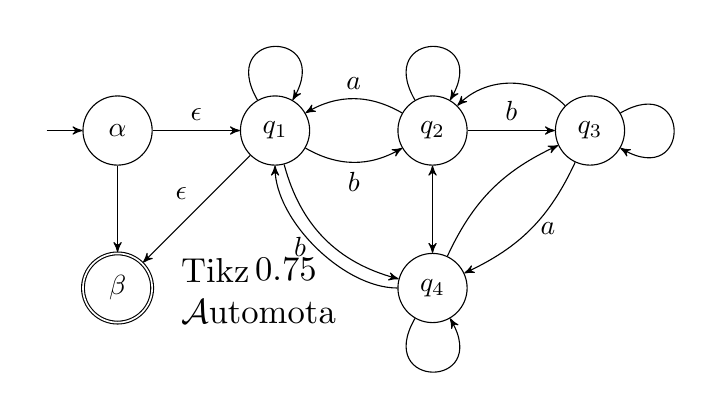
\begin{tikzpicture}

            % nodes
            \node[state] (q1) {$q_1$};
            \node[state, right of=q1] (q2) {$q_2$};
            \node[state, right of=q2] (q3) {$q_3$};
            \node[state, below of=q2] (q4) {$q_4$};
            \node[state, initial, left of=q1] (qA) {$\alpha$};
            \node[state, accepting, below of=qA] (qB) {$\beta$};

            % text node
            \node [right of=qB, align=left, xshift=-6px, yshift=-1px, scale=1.25] (text) {Tikz$\,\arrow$\\$\mathcal{A}$utomota};

            \draw (q1) edge[below, bend right] node{$b$} (q2)
            (q2) edge[above, bend right] node{$a$} (q1)
            (q2) edge[above] node{$b$} (q3)
            (q3) edge[right, bend left=20] node{$a$} (q4)
            (q4) edge[left, bend left=45, looseness=0.8] node{$b$} (q1)

            % null transitions
            (q1) edge[right, bend right] node{$\varnothing$} (q4)
            (q2) edge[<->, left] node{$\varnothing$} (q4)
            (q4) edge[left, bend left=20] node{$\varnothing$} (q3)
            (q3) edge[bend right=45, above] node{$\varnothing$} (q2)
            (qA) edge[above] node{$\epsilon$} (q1)
            (q1) edge[above left] node{$\epsilon$} (qB)
            (qA) edge[left] node{$\varnothing$} (qB)
            (q1) edge[loop above, in=60, out=120, looseness=6] node{$\varnothing$} (q1)
            (q2) edge[loop above, in=60, out=120, looseness=6] node{$\varnothing$} (q2)
            (q3) edge[loop right, in=-30, out=30, looseness=6] node{$\varnothing$} (q3)
            (q4) edge[loop below, in=-60, out=-120, looseness=6] node{$\varnothing$} (q4)
            ;

        \end{tikzpicture}
    \end{figure}
\end{document}